\documentclass[aps,prd,10pt,onecolumn,nofootinbib,superscriptaddress,floatfix]{revtex4-2}

\usepackage[T1]{fontenc}
\usepackage{lmodern}
\usepackage[utf8]{inputenc}
\input{glyphtounicode}
\pdfgentounicode=1
\usepackage{amsmath,amssymb,mathtools}
\usepackage{bm}
\usepackage{graphicx}
\usepackage{placeins}
\usepackage{hyperref}

\hypersetup{
  colorlinks=true,
  linkcolor=blue,
  citecolor=blue,
  urlcolor=blue
}

\begin{document}
\raggedbottom

\title{Can a Wormhole Induce a Monopole?}

\author{Sergei Slobodov}
\email{sergei@slobodov.com}
\noaffiliation

\date{\today}

\begin{abstract}
Could a body orbiting near one mouth of a traversable wormhole make the mass
seen near the other mouth rise and fall?  Monopole rigidity precludes this
possibility.  In the Maxwell case, source motion cannot induce a time-varying
monopole across the throat, though higher time-varying multipoles can be
present.  The same holds for gravity at linear order.  This argument is local
and requires neither a compact interior nor a specific asymptotic structure.
A cumulative monopole change requires matter to cross the measuring surface
or, at second order, gravitational-radiation flux.
\end{abstract}

\maketitle

% ============================================================
\section{Introduction}
\label{sec:introduction}
% ============================================================

A wormhole can support a static monopole (mouth mass) at each end.  In this note
we show that a body on an eccentric orbit around one mouth cannot make this
monopole dynamic, contrary to the proposal by Dai and Stojkovic (DS)
\cite{DaiStojkovic2019Observing}.  The DS setup is two Schwarzschild exteriors
connected along a sphere of radius $R$ excised from each. They place a body
of mass $\mu$ at radius $A$ in one exterior, solve a static matching problem,
then interpret the resulting family of solutions as a dynamical evolution of
an orbiting mass.  DS and Simonetti et al. take this approach to produce a
periodic $1/r^2$ acceleration \cite{SimonettiEtAl2021SensitiveSearches}.
The validity of this approach has been discussed in
Refs.~\cite{Krasnikov2020CommentObserving,DaiStojkovic2020ReplyObserving}.

However, the set of static solutions and the dynamical orbit pick different
constraints.  The DS version fixes the potential difference between the two 
asymptotic ends, while the free evolution lets it float because the flux 
through each mouth is fixed.  In the gravitational equivalent, imposing the 
same time coordinate at both ends at all times makes the observer-side 
Schwarzschild mass perturbation time-dependent, contrary to the vacuum 
momentum constraint.  This is monopole rigidity: the monopole measured 
at the observer end does not track the source's instantaneous orbital radius.

The conclusion does not assume spherical source motion.  On the spherical
background used by DS, the monopole projection evolves independently of all
higher harmonics.  Additional monopole components are either a changing mass,
which requires energy flux, or pure gauge, in which case $h_{tt}$ alone does
not define an observable acceleration.

We first establish the exact Maxwell charge balance for a single end and use
the DS electrostatic family to show how static matching can move between flux
sectors.
We then take the DS gravitational coefficient as given and test its proposed
time dependence directly, separate the gauge and higher-multipole sectors, and
bound the leading surviving quadrupole in a standard thin-shell model.
We use geometrized units $G=c=1$, write $r_g=2M$, and work to first order in
$\mu/M\ll1$.

% ============================================================
\section{Maxwell: charge at one end}
\label{sec:maxwell}
% ============================================================

The replacement $A\to A(t)$ in the DS electrostatic family does not produce a
solution of Maxwell's equations: each end charge stays constant unless current
crosses its measuring worldtube.
Let $F$ be the electromagnetic field strength, $j$ the electric current
one-form, and $\star$ the Hodge dual.
For a closed measuring surface $S$, define
\begin{equation}
  Q[S]=\frac{1}{4\pi}\int_S\star F.
  \label{eq:maxwell-charge}
\end{equation}
Let $S_t$ be a family of closed measuring surfaces and let
$\mathcal T=\bigcup_{t\in[t_1,t_2]}S_t$ be the timelike worldtube they sweep
out, with $\partial\mathcal T=S_{t_2}-S_{t_1}$.  Integrating
$d\star F=4\pi\star j$ over $\mathcal T$ and applying Stokes' theorem gives
\begin{equation}
  Q[S_{t_2}]-Q[S_{t_1}]=\int_{\mathcal T}\star j.
  \label{eq:maxwell-balance}
\end{equation}
Thus the end charge is constant whenever no electric current crosses
$\mathcal T$; the surfaces $S_t$ need not bound compact regions.

Frolov and Novikov obtained this balance for wormholes and emphasized that
external charge motion leaves the handle flux unchanged until charge passes
through it \cite{FrolovNovikov1990PhysicalEffects}.

DS glue two copies of flat space outside a sphere of radius $R$, put a charge
$q$ at $r_1=A$ in one copy, and observe the field at $(r_2,\theta_2)$ in the
other \cite{DaiStojkovic2019Observing}.  Let $c_1$ and $c_2$ be the asymptotic
potentials at the two ends.  Matching the potential
and its normal derivative at the throat gives
\begin{equation}
  V_2=c_2+\sum_{\ell\ge0}\frac{B_\ell}{r_2^{\ell+1}}
       P_\ell(\cos\theta_2),
  \quad
  B_{\ell\ge1}=q\,\frac{2\ell+1}{2(\ell+1)}
       \frac{R^{2\ell+1}}{A^{\ell+1}},
  \quad
  B_0=\frac{qR}{2A}+\frac{R}{2}(c_1-c_2),
  \label{eq:ds-multipoles}
\end{equation}
where $P_\ell$ is a Legendre polynomial.  The source position fixes every
$\ell\ge1$ coefficient.  It does not fix the monopole because the relative
potential $c_1-c_2$ is independent boundary data.

The free coefficient has direct physical meaning: in the normalization of
Eq.~\eqref{eq:maxwell-charge}, the observer-side charge is $Q_2=B_0$.  Its
second term, $\tfrac{R}{2}(c_1-c_2)$, does not involve the source and survives
with no charge present in either copy, Wheeler's ``charge without charge''
\cite{MisnerWheeler1957ClassicalPhysics}; the coefficient $R/2$ is the
end-to-end capacitance.  The potential difference between the ends is the work
per unit charge required to move charge from one to the other.

The choice between fixing charge and fixing potential is familiar from
conductors \cite[Ch.~2]{JacksonClassicalElectrodynamics}.  Setting
$c_1=c_2$ fixes equal potentials at the two asymptotic ends and gives
\begin{equation}
  Q_2(A)=B_0=\frac{qR}{2A}.
  \label{eq:ds-electric}
\end{equation}
Imposing equal end potentials anew at every $A$ selects a different static
charge.  During an evolution, however, the source does not cross the
observer-side measuring worldtube, so Eq.~\eqref{eq:maxwell-balance} keeps
$Q_2=B_0$ constant while the potential difference adjusts.

DS correctly obtain $Q_1+Q_2=q$, with $Q_1$ the source-side flux, but interpret
only the sum as conserved
\cite[discussion following Eqs.~(9) and (10)]{DaiStojkovic2019Observing}.
Applying Eq.~\eqref{eq:maxwell-balance} to a measuring worldtube in each
exterior gives $\dot Q_1=\dot Q_2=0$ as long as the charge crosses neither
worldtube.  Thus both end charges are separately conserved.

The balance law constrains only the monopole; fixed flux does not eliminate the
higher-multipole cross-mouth field.
The compensating harmonic field required to preserve the throat flux was
identified by Frolov and Novikov, and the corresponding fixed-flux point-charge
problem was formulated by Krasnikov
\cite{FrolovNovikov1990PhysicalEffects,Krasnikov2008ElectrostaticInteraction}.
Figure~\ref{fig:fixed-sector-field} visualizes the $B_0=0$ member of
Eq.~\eqref{eq:ds-multipoles}, for which all observer-side field is carried by
$\ell\ge1$.

\begin{figure}[!b]
  \centering
  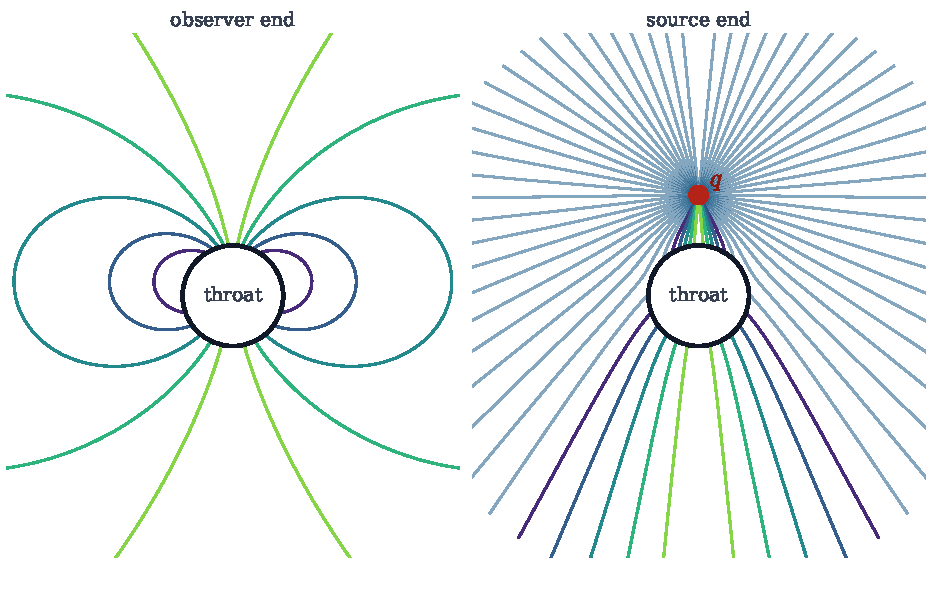
\includegraphics[width=0.82\textwidth]{figures/fig_thinshell_fixed_monopole_flux_v7.pdf}
  \caption{The zero-flux member of Eq.~\eqref{eq:ds-multipoles}: $B_0=0$,
  requiring $c_2-c_1=q/A$.  The black circles represent the same throat sphere
  in the two exterior charts.  Field lines cross the throat but return through
  another angular band, giving zero net flux.  The
  observer-side field is nonzero and contains only $\ell\ge1$ terms.}
  \label{fig:fixed-sector-field}
\end{figure}
\FloatBarrier

When both mouths lie in the same asymptotic region, there is no pair of end
potentials to equate.
Frolov and Novikov represent the free handle-flux mode by a nonpotential field
with circulation $\oint_\gamma\mathbf E\mathbin{\cdot}d\mathbf l$ around a
loop $\gamma$ through the throat and back
\cite{FrolovNovikov1990PhysicalEffects}.  The circulation need not vanish
because the loop bounds no surface.  Setting it to zero is the analogue of
setting $c_1=c_2$ in the two-ended model.  Neither choice enters the local
balance~\eqref{eq:maxwell-balance}: without current across the measuring
worldtube, the end charge is constant.

\FloatBarrier

% ============================================================
\section{The Dai--Stojkovic gravitational signal}
\label{sec:gravity}
% ============================================================

The replacement $A\to A(t)$ made by DS and Simonetti et al. does not produce a
vacuum solution
\cite{DaiStojkovic2019Observing,SimonettiEtAl2021SensitiveSearches}.  The
observer-side coefficient $b=\mu R/A$ is a Schwarzschild mass shift, which the
vacuum equations require to be constant.  The proposed first-order monopole
signal is therefore absent.

\subsection{The observer-side monopole}

DS join two copies of the Schwarzschild exterior,
\begin{equation}
  d\bar s^2=-f(r)dt^2+f(r)^{-1}dr^2+r^2d\Omega^2,
  \qquad f(r)=1-\frac{r_g}{r},
  \label{eq:background}
\end{equation}
at $r=R>r_g$.  A source of mass $\mu$ is placed at $r_1=A>R$ in one
exterior.  At fixed $A$, DS obtain $b=\mu R/A$
\cite{DaiStojkovic2019Observing}.  In a later arXiv revision they set
$b_{rr}=b_{tt}=b$ \cite{DaiStojkovic2019ObservingV3}, so the observer-side
vacuum perturbation is
\begin{equation}
  h^{\mathrm{obs}}_{tt}=\frac{2b}{r_2},
  \qquad
  h^{\mathrm{obs}}_{rr}=\frac{2b r_2}{(r_2-r_g)^2},
  \qquad
  b=\frac{\mu R}{A}.
  \label{eq:ds-observer-mode}
\end{equation}
Since $r_g=2M$, this is exactly
$h^{\mathrm{obs}}_{\alpha\beta}=b\,\partial_M\bar g_{\alpha\beta}$.  More
generally, every first-order monopole in a connected Schwarzschild vacuum
region has the form
\begin{equation}
  h^{\ell=0}_{\alpha\beta}
  =\delta M\,\partial_M\bar g_{\alpha\beta}
   +\mathcal L_\eta\bar g_{\alpha\beta},
  \qquad \partial_t\delta M=0,
  \label{eq:l0-classification}
\end{equation}
where $\eta^\alpha$ is a gauge vector
\cite{MartelPoisson2005SchwarzschildPerturbations}.  The DS coefficient $b$ is
therefore the observer-side mass perturbation, whose far-field acceleration is
$-b/r_2^2$.  The associated time-translation charge on any round sphere is $b$;
at an asymptotically flat end it agrees with the Arnowitt--Deser--Misner mass
variation \cite{IyerWald1994NoetherCharge}.

Under the replacement $A\to A(t)$, Eq.~\eqref{eq:ds-observer-mode} is the
linearization of Eq.~\eqref{eq:background} with
$f(r_2)$ replaced by
$F(t,r_2)=1-2[M+b(t)]/r_2$.  For this metric the exact mixed component, and
hence its first-order part, is
\begin{equation}
  \delta G^{r}{}_{t}=G^{r}{}_{t}
  =-\frac{\partial_t F}{r_2}
  =\frac{2\dot b}{r_2^2}
  =-\frac{2\mu R\dot A}{A^2r_2^2}.
  \label{eq:momentum-constraint}
\end{equation}
For $\dot A\ne0$, Eq.~\eqref{eq:momentum-constraint} violates the observer-side
vacuum equation $G^{r}{}_{t}=0$.  Hence $b=b_0$ throughout the orbit.

For periapsis $r_p$ and apoapsis $r_a$, DS infer
\begin{equation}
  |\Delta a_{\mathrm{DS}}|
  =\mu R\left(\frac{1}{r_p}-\frac{1}{r_a}\right)\frac{1}{r_2^2}.
  \label{eq:ds-signal}
\end{equation}
The same $b_0$ applies at both orbital phases, so the $A(t)$-dependent monopole
modulation proposed in Eq.~\eqref{eq:ds-signal} is
\begin{equation}
  |\Delta a^{(A)}_{\ell=0}|=0.
  \label{eq:monopole-zero}
\end{equation}

The gauge term in Eq.~\eqref{eq:l0-classification} is the other possible
$\ell=0$ contribution.  If a completion moves the apparent time dependence
into this term, it changes coordinates rather than the mass.  An acceleration
must then be derived from a gauge-invariant observable rather than from
$h_{tt}$ alone.

With a source, the same constraint gives the balance law on a measuring sphere
$S_r$ at radius $r_2$,
\begin{equation}
  \dot b=\oint_{S_r}\delta T^{r}{}_{t}\,dS.
  \label{eq:mass-flux}
\end{equation}
The DS measuring worldtube lies in vacuum, so Eq.~\eqref{eq:mass-flux} gives
$\dot b=0$.  The monopole is fixed
by the body's conserved Killing energy rather than by its instantaneous
radius.  Matter crossing the measuring sphere can change the monopole at first
order; gravitational-wave energy flux can do so at second order
\cite{BondiVanderBurgMetzner1962Gravitational,Sachs1962Asymptotic}.

\subsection{Higher multipoles}

Equation~\eqref{eq:monopole-zero} concerns only the monopole.  Nonspherical
source motion also excites higher multipoles.  In linear perturbation theory
about Schwarzschild, different $\ell$ sectors decouple, so they leave the
monopole result unchanged.

For an isolated system, the even-parity $\ell=1$ perturbation describes
center-of-mass motion, which is constant in the asymptotic barycentric frame;
the odd-parity $\ell=1$ perturbation is the conserved total angular momentum
\cite{MartelPoisson2005SchwarzschildPerturbations}.  Orbital time dependence
therefore begins with the quadrupole \cite{Thorne1980Multipole}.

The quadrupolar acceleration relative to the proposed monopole scale is
\begin{equation*}
  \frac{a_2}{a_{\mathrm{DS}}}
  \sim C_2\left(\frac{R}{A}\right)^2
  \left(\frac{R}{r_2}\right)^2.
\end{equation*}
Here $C_2$ is a model-dependent quasistatic transfer coefficient.  The static
stiff-shell model of Cardoso et al. gives $C_2\leq5/2$, an order-unity
benchmark \cite{CardosoEtAl2017LoveNumbers}.  For
$r_2\simeq1000\,\mathrm{AU}$ as in the Sgr~A*/S2 estimate and a favorable
$A\sim R\sim r_g$ satisfying $R-r_g\gg\mu$, the ratio is of order $10^{-8}$.

% ============================================================
\section{Conclusion}
\label{sec:conclusion}
% ============================================================

The DS calculation gives a family of static geometries labeled by the source
radius.  Its observer-side coefficient is a Schwarzschild mass perturbation.
Promoting the label to $A(t)$ violates the vacuum momentum
constraint, so the proposed time-dependent monopole is not a source-free
first-order solution.  Nonspherical components cannot change
the monopole equation, and a gauge completion would remove rather than rescue
the claimed mass observable.

The Maxwell model makes the sector distinction explicit: equal-potential
static solutions at different $A$ have different end flux, whereas an
evolution with no current through the measuring worldtube preserves it.
Gravity reaches the corresponding conclusion independently through the vacuum
monopole constraint.  In either case, an end charge is not an instantaneous
response coefficient.  The first physical orbital modulation is therefore
quadrupolar; in the stiff-shell benchmark above, its amplitude is of order
$10^{-8}$ of the proposed Sgr~A*/S2 monopole scale.  Waves and
dynamical throat modes require a separate dynamical model.

\begin{acknowledgments}
The author thanks Ilia Slobodov for helpful discussions.
\end{acknowledgments}

\section*{Artificial Intelligence Use Statement}

The author used OpenAI ChatGPT/Codex and Anthropic Claude as interactive
assistants for brainstorming, mathematical and editorial critique, prose
revision, consistency checks, reference searches, and figure preparation.  All
arguments, calculations, citations, figures, and conclusions were reviewed and
revised by the author, who is solely responsible for the manuscript.

\bibliographystyle{apsrev4-2}
\bibliography{references}

\end{document}
